\documentclass[conference]{IEEEtran}

\usepackage{cite}
\usepackage{url}
\usepackage{calligra}
\usepackage{amsmath,amssymb,amsfonts}
\usepackage{algorithmic}
\usepackage{textcomp}
\usepackage{xcolor}

\usepackage{graphicx}
%Path relative to the main .tex file 
\graphicspath{ {./images/} }

\usepackage{verbatim} %for multiline comments

\setlength{\marginparwidth}{2cm}
\usepackage{todonotes} % for TODOs

\def\BibTeX{{\rm B\kern-.05em{\sc i\kern-.025em b}\kern-.08em
    T\kern-.1667em\lower.7ex\hbox{E}\kern-.125emX}}
    
%%% For algorithms 
\usepackage[linesnumbered,ruled,vlined]{algorithm2e}
\SetKwInput{KwInput}{Input}                % Set the Input
\SetKwInput{KwOutput}{Output}              % set the Output
%%% End Algos

\begin{comment}
% make custom headings
\usepackage{titlesec}

\titleformat{\section}
  {\normalfont\fontsize{12}{17}\sffamily\bfseries}
  {\thesection}
  {1em}
  {}
\end{comment}

\begin{document}

\title{\rule{\textwidth}{1pt} Adversarial Training - Theory and Algorithms
\vspace{-1cm} \rule[15pt]{\textwidth}{1pt}}

\author{\IEEEauthorblockN{Moritz Sch{\"u}ler}
\IEEEauthorblockA{\textit{dept. of Informatics} \\
\textit{Technical University Munich}\\
Munich, Germany\\
moritz.schueler@tum.de}
\vspace{-1cm}
}

\maketitle

\begin{IEEEkeywords}
  ML, Adversarial Training, robustness
\end{IEEEkeywords}

\section*{Abstract}
Adversarial training is a technique that tries to achieve robust deep networks. Robustness in a sense, that perturbing the input does not lead to a false prediction of the model. The presented paper provides a conceptual introduction to adversarial training as well as a review of current methods. While it's not possible to discuss all adversarial training approaches, some recent advancements are described in detail and their advantages and disadvantages are highlighted. Additionally, possible directions for future research are presented.

\section{Introduction}

Many standard trained neural networks achieve high, even super human performance in a wide range of tasks. However, they can be easily fooled with the help of adversarial examples. Adversarial examples are generated by applying small perturbations to valid input data, which lead a classifier to change its prediction. Even though neural networks apply a non-linearity at each layer to allow for complex decision boundaries, \cite{b27} shows that the decision boundaries are excessively linear in most areas. This can be seen in figure 1 for a trained CIFAR10 model. \\

\begin{figure}[ht]
  \centering
  \vspace{-0.7cm}
  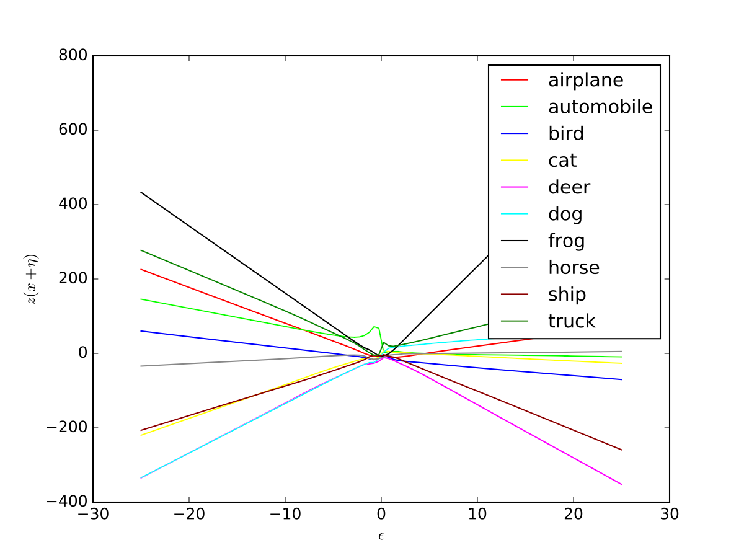
\includegraphics[scale=0.35]{CIFAR10-decision_boundary.png}
  \vspace{-0.35cm}
  \label{fig: Decision boundary of a neural network}
  \caption{Decision boundaries of a neural net trained on CIFAR10 \cite{b27}}
  \vspace{-0.2cm}
\end{figure}

Moreover, \cite{b2} demonstrated why linear decision boundaries are problematic for robustness. In figure 2 on the left a perfect linear classifier is displayed. However, in the middle the presence of adversarial examples is shown. A small perturbation, bounded by shaded box around each sample, allows two samples to become adversarial (marked by a red star). Lastly, on the right a decision boundary for an adversarial trained network is displayed which is robust against small perturbations of the input data. Further, \cite{b6} demonstrated the need for robust models in practice, as simply putting a sticker on a stop sign fooled the network to recognize it as a speed limit. These problems lead to research how to defend against, but also how to generate adversarial examples. \\

\begin{figure}[ht]
  \centering
  \vspace{-0.6cm}
  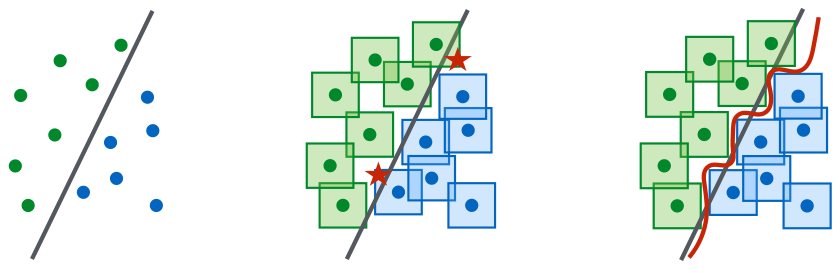
\includegraphics[scale=0.29]{decision_boundaries.png}
  \vspace{-0.45cm}
  \label{fig: standard and adversarial decision boundaries}
  \caption{"A conceptual illustration of standard vs. adversarial decision boundaries" \cite{b2}} 
  \vspace{-0.2cm}
\end{figure}

The latter one is called adversarial attack and focuses on finding a model that can generate adversarial examples by applying small perturbations to an input datapoint. Adversarial training on the other side is an approach to harden the model against adversarial attacks by training on adversarial examples of the input data. It tries to find perturbed samples that get wrongly classified, include them into the training and afterwards adjust the model parameters to get a correct prediction. In figure 2 this means that the red classifier was trained with samples that lay on the edge of the surrounding boxes of the data points, leading to a robust decision boundary for these samples. \\
This paper aims at providing a comprehensive introduction to adversarial training and a review on current approaches. More precisely, it focuses on standard adversarial training, especially from the view of robust optimization. This includes universal adversarial training as well as margin maximization. However, there exist a variety of other approaches to increase the robustness of classifiers. The authors of \cite{b19, b20} use logit pairing, where a regularization is applied to the logits. \cite{b23} use ensemble methods to enhance robustness, whereas \cite{b21, b22} in contradiction distill the model. Another view on increasing robustness is calculating a distance within the prediction does not change. This research area is about certifiable robustness \cite{b30}. Furthermore, latent representations are also examined to increase robustness \cite{b31}. \\
In the next section properties and types of adversarial attacks are presented. How to defend against them is part of the third section about the theoretical concept of adversarial training. Specific methods and their properties are shown in section 4, while section 5 gives a comparison of the discussed approaches. The last section specifies possible directions for future research.

\section{Adversarial Attacks}

The task of adversarial attacks is to find a model that generates samples for a given classifier, such that its prediction is wrong. Let $x$ denote a sample from the distribution of the training data which classifies as $y$ with high probability $p(y|x)$. An adversarial example is now characterized by adding a small perturbation $\tilde{r} < \epsilon$ to $x$, such that the classification of $\tilde{x} = x + \tilde{r}$ results in $y'$ with high probability $p(y'|\tilde{x})$, but having a different predicted class $y' \neq y$. Here $\epsilon$ defines the maximum perturbation distance from the original sample, i.e. the boxes in figure 2. Another kind of adversarial example is described by having a very large distance to the actual sample but still resulting in a high probability of $p(y'|\tilde{x})$. However, the latter one will not be part of this paper. \\
The objective for adversarial attacks is to find a perturbation $\delta$, such that the loss of the classification model $l(f_{\theta}(x_i), y_i)$ is maximized. Usually a threat model $\Delta$ is used for this, which tries to find a $\delta$ within some lp-norm smaller than $\epsilon$. Here $\epsilon$ is a hyperparameter that specifies the strength of the attack. 
\begin{align*}
  \max_{\delta \in \Delta} & \quad l(f_{\theta}(x_i + \delta), y_i)  \\
\Delta &= \{\delta : ||\delta||_p \leq \epsilon\} \quad s.t. \quad \epsilon > 0
\end{align*}

Finding the maximum can easily be done via projected gradient ascent for the input x. However, accessing the gradient information is not always possible. This lead to the development of several different attacks. If a white box attack via gradient ascent is not feasible, the property that adversarial examples are model-agnostic can be used. The idea is to perform a gray box attack by training an own model on the data and using its gradient information to generate an attack. Lastly, if no gradient information is available at all, one can try to find gradient free perturbations, i.e. adding random noise and generate a black box attack. \\
Adversarial attacks can be further divided into targeted and non-targeted attacks. The first one tries to change the prediction of a given sample $x$ to a specified target label $y$, whereas the latter one only tries to change the prediction to some other class. Lastly, a distinction can be made between finding perturbation for each given sample $x$ or finding a single perturbation over all $X$, that achieves a missclassification for many $x$. In this work, we focus on white box and non-targeted attacks, as for training the gradient is known and robustness should be increased generally and not for a specific class. 

\section{Adversarial Training}

Adversarial training is a training form for neural networks that tries to achieve higher robustness against adversarial attacks by using the adversarial examples belonging to the training data for training. By doing so it tries to increase the non-linearity of the decision boundary, as seen in figure 2. \\
The training objective for adversarial training is a two step problem. Basically we are trying to minimize the loss of an adversarial attack model. So in the first step the inner maximization is approximated by some threat model, similar or equal to the ones presented for adversarial attacks. Afterwards the outer minimization is solved by a variant of gradient descent on the model parameters $\theta$. \\
Let $x$ be a training sample and $f_{\theta}$ be the classifier. First, we are solving a maximization of the classification loss, i.e. cross entropy loss, for a perturbation $\delta$ coming from a threat model $\Delta$ like in the case of an adversarial attack. This is done for each training sample separately and the "worst-case" losses are summed up. Afterwards, as in standard training, this summed loss is minimized via gradient descent on the model parameters $\theta$. This is done via mini-batches for several epochs as in usual training of neural networks.
\begin{align*}
  \min_{\theta} & \sum_i \max_{\delta \in \Delta} \space l(f_{\theta}(x_i + \delta), y_i)  \\
\Delta & = \{\delta : ||\delta||_p \leq \epsilon\} \quad s.t. \quad \epsilon > 0
\end{align*}
However, calculating the gradient of this objective function is not straight forward because of the max operation. Luckily, by applying Daskin's Theorem the problem can be simplified. \\

\textbf{Danskin's Theorem}: The (sub)gradient of a function containing a max term can be found by taking the gradient at the point of the maximum $\delta^{*}$.
\begin{align*}
  \nabla_{\theta} \max_{||\delta|| \leq \epsilon} l(f_{\theta}(x_i + \delta), y_i) = \nabla_{\theta} l(f_{\theta}(x_i + \delta^{*}(x_i)), y_i)
\end{align*}

Theoretically, the theorem has some required conditions, which might not hold in the case of adversarial training, i.e. having a convex loss function $l(f_{\theta}(x_i + \delta), y_i)$ or that it only holds for the exact maximum. The trade-off emerging from that is, that the robustness depends on the precision of the maximum, but using a multi-step approach for a better approximation slows down the overall process. \\
The two main challenges, which are addressed by different presented methods in the next section are finding a better or faster solution for the generation of the adversarial training samples, as well as finding a way to be robust against all threat models. Because research showed that models are very robust against the threat model they were trained on, but lack robustness against other attacks.

\section{Methods}

In practice, several approaches have been studied to combat the mentioned challenges. In this section some recent methods and their peculiarities are presented. Especially the objective function, as well as the threat model used by the approaches are discussed.

\subsection{Robust Optimization - Standard Adversarial Training} \label{Robust Opti}

The standard approach on adversarial training stems from the view of robust optimization. It formulates the training process as a saddle point problem where the adversarial attack tries to maximize the loss whereas the network tries to minimize it. This is exactly the formulation presented in the previous section. Here we want to elaborate on the differences in threat models that are used to generate the adversarial examples. \\
The very first model was introduced by \cite{b9} in 2014, where the adversarial example $\tilde{x}$ is found by taking a single step into the gradient direction of defined length $\epsilon$. This technique is called fast gradient sign method (FGSM) and is the basis for most further optimization.
\begin{align*}
x^{t+1} = x + \epsilon * sgn(\nabla_x L(\theta,x,y)))
\end{align*}
The second threat model belonging to the family of robust optimization is the multi-step projected gradient descent method (K-PGD), created by \cite{b28}. Here instead of going a single big step into the gradient direction, we are moving $k$ (hyperparameter) smaller steps of size $\alpha$ into the gradient direction. Important is that if an update leads to stepping out of the $\epsilon$ ball, we need to project back, which is done by the projection function $\Pi$. This leads to a better approximation of the inner maximization but longer training times. This method is still the most widely used approach for training a robust neural network. 
\begin{align*}
  x^{t+1} &= \Pi_{x+S} (x^t + \alpha \space sgn(\nabla_x L(\theta,x,y)))
\end{align*}
Note that setting $k=1$ and $\alpha=\epsilon$ this resembles FGSM, so it can also be seen as a generalzation of the previous method. \\
Another approach that improves on FGSM brought in by \cite{b5} was Free Training. The main idea is to use the gradients from the outer minimization at time t for the gradient ascent of the adversarial example at time t+1. To reach a comparable robustness as K-PGD, each mini-batch is replayed $m$ times. Additionally, a new mini-batch is warm started by the perturbation of the previous one. To stay efficient the number of epochs is lowered accordingly, resulting in nearly no overhead compared to traditional training.
Fast Training, by \cite{b3}, further improved on Free Training by using FGSM with random initialization and getting rid of the mini-batch replay. They showed that the important ingredient to be comparably robust is only allowing for radomized initialization for the perturbation and thus could drastically speed up the training process. \\
% maybe put at the end of section or at beginning of comparison
Additionally, several training settings can influence the performance. Using another optimizer like momentum empirically leads to better adversarial examples \cite{b29}. Furthermore, increasing the capacity of a model can lead to improved robustness, as shown by \cite{b2}. Therefore, there is not one approach that works for all problems. Instead, one should try different training setups, including different threat models.

\begin{comment}
Two more approaches, using the saddle point formulation, improve robustness by applying a regularization. \cite{b8} indirectly regularizes the gradient norm by perturbing the samples as well as the labels. The advantage of a small gradient norm is that the surface of the loss function gets very flat, making it hard for gradient-based attacks to find a maximum. Another way of regularization by \cite{b25} is applied on the perturbations itself. The idea is to keep the norm of the perturbation small to be robust against various threat models.

\begin{itemize}
  \item FGSM \cite{b9}
  \item K-PGD \cite{b2}: multistep projected FGSM
  \item Free Training \cite{b5}: Mini-batch replay + warm start
  \item Fast Training \cite{b3}: FGSM with random init
  \item GradAlign \cite{b7}: FGSM with Gradient Alignment (refutes random init)
  \item SLAT \cite{b26}: Using latent adversarial perturbations
  \item Bilateral Adversarial Training \cite{b8}: regularize gradient norm
  \item Dual Head Adversarial Training \cite{b24}: use one hat for robustness
  \item Lagrangian objective function \cite{b25}: use lagrangian regularization
\end{itemize}
\end{comment}

\subsection{Universal Adversarial Training}
Universal Adversarial Training (UAT) is a method that does not try to find a perturbation for each single sample but rather a global perturbation that fools the classifier for many samples, hence the name universal. The difference can also be seen in the objective function which iterates over all samples in the inner term. As it tries to find a universal perturbation it is more constrained than the standard approach and hence leads to a less robust model, while reducing the training time. \\
In \cite{b4} the authors formulate this as a min-max optimization problem:
\begin{align*}
  \min_{\theta} \max_{\delta \in \Delta} \space \frac{1}{N} \sum_{i=1}^N \space \hat{l}(f_{\theta}(x_i + \delta), y_i) \quad s.t. \quad ||\delta||_p \leq \epsilon \\
  \text{with} \quad \hat{l}(f_{\theta}(x_i + \delta), y_i) = \min \{l(f_{\theta}(x_i + \delta), y_i), \beta \} \\
\end{align*}
where $\theta$ represents the trainable parameters of the neural network, $x_i$ the training samples, $y_i$ the training labels, $\delta$ the universal perturbation and $\hat{l}(\cdot)$ the loss function. Note, that $\delta$ is again bounded by an lp-ball of size $\epsilon$ and calculated by a threat model $\Delta$. For this all presented models of the previous section can be used. Further notice, that the loss function $\hat{l}(\cdot)$ is bounded from above by a hyperparameter $\beta$. This is crucial because it hinders a single sample to dominate the average loss in the inner loop. Otherwise "a perturbation, that causes missclassification of just a single sample can maximize [the inner term] by forcing the average loss to infinity"\cite{b4}. \\
A recent advancement on this formulation is done by \cite{b11}. The key idea is to relax the constraints and thus get stronger attacks during training. Particularly, the authors show, a network trained on class-wise universal perturbations (CW UAT) exhibits higher robustness to universal perturbation attacks.

\begin{comment}

\begin{itemize}
  \item universal Adversarial Training with class-wise perturbations \cite{b11}
  \item Deep Fool
  \item Defending Against Universal Perturbations With Shared Adversarial Training \cite{b12}
  % -> 20 times slower than normal training
  \item Defense against Universal Adversarial Perturbations \cite{b13}
  \item Universal Adversarial perturbations \cite{b10}
\end{itemize}

\end{comment}

\subsection{Margin Maximization}
Margin Maximization is a method that tries to maximize the distance between each sample and its nearby decision boundary. Intuitively this makes the model more robust as an adversarial example is a slight perturbation of a datapoint that changes the model outcome and this is usually a sample that is very close to a decision boundary. Thus, by maximizing said distance, also called margin, it is harder to generate adversarial examples and therefore increasing robustness to adversarial attacks. \\
One formulation, used by \cite{b15}, is to describe the margin $d_{f,x,\{i,j\}}$ by the smallest perturbation $\delta$ to a decision boundary $D_{\{i,j\}}$,
\begin{align*}
  d_{f,x,\{i,j\}} \triangleq \min_{\delta} \parallel \delta \parallel_p \quad \text{s.t.} \quad f_i(x+\delta) = f_j(x+\delta) \\
  \text{with} \quad D_{\{i,j\}} \triangleq \{x|f_i(x) = f_j(x)\}
\end{align*}
where $f(\cdot)$ is the model depending on $\theta$ and $\parallel \cdot \parallel_p$ is any $l_p$ norm. The objective is then to maximize the margin to all decision boundaries for every training sample $x_k$ by adjusting the model parameters $\theta$. This leads to the overall loss function,
\begin{align*}
  \min_{\theta} \sum_k \text{\calligra A}_{i \neq y_k} \max \{0, \gamma + d_{f,x_k,\{i,y_k\}} \space sgn (f_i(x_k) - f_{y_k}(x_k)) \\
  \text{with} \quad \text{\calligra A} = \{\sum, \max\}
\end{align*}
Here the loss is summed over all classes $k$ and aggregated for the multiclass setting by an aggregation operator \text{\calligra A}. The $sgn(\cdot)$ ensures the stronger penalization for wrongly classified samples and $\gamma$ is a hyperparameter, specifying the minimum margin. The authors show that for a linear approximation of $d_{f,x,\{i,j\}}$ a closed form solution of the objective exists and can be used for adversarial training (For further reference, this approach is called "Large Margin"). \\
A different formulation of the problem is given by \cite{b1}. Here the margin $d_\theta(x_i, y_i)$ is defined by the smallest successfull perturbation $\delta^*$, 
\begin{align*}
  d_\theta(x,y) & = ||\delta^*|| = min ||\delta|| \\ 
  \text{s.t.} \quad \delta: & L_\theta^{01}(x+\delta, y) = 1
\end{align*}
where $L_\theta^{01}$ is the 0-1 loss inidating a classification error. The idea, proposed by the authors, is to maximize the average margin over the data. Hence, they name it Max-Margin Adversarial training (MMA). For this, the problem is divided into maximizing the margin for already correctly classified samples $S_{\theta}^{+}$ and correcting the prediction for all wrongly classified datapoints in $S_{\theta}^{-}$.
\begin{align*}
  \min_{\theta} \Big\{ \sum_{i \in S_{\theta}^{+}} & \max \{0, d_{max} - d_\theta(x_i, y_i)\} + \beta \sum_{j \in S_{\theta}^{-}} \mathcal{J}_\theta (x_j, y_j) \Big\}
\end{align*}
Here $\beta$ controls the trade-off between maximizing the margin and correcting wrong predictions. $\mathcal{J}(\cdot)$ is a standard classification loss, like cross entropy and $d_{max}$ is a hyperparameter, specifying the minimum margin. Additionally, $d_{max}$ also leads the learning to focus on margins that are smaller as itself, because it acts as a threshold for the margin $d_\theta(x_i, y_i)$ inside the hinge loss. In contrast to \cite{b15}, finding the smallest margin in this work is done via a variant of K-PGD, presented in \ref{Robust Opti}.

\begin{comment}
\begin{itemize}
  \item MMA Training: Direct input space margin maximization through adversarial training\cite{b1}
  \item Large Margin Deep Networks for Classification \cite{b15}
  
  \item Deep Defense: Adversarial Margin Maximization Networks \cite{b14}
  \item Margin Maximization for Robust Classification using Deep Learning \cite{b16}
  \item MACER: Attack-free and scalable robust training via maximizing certified radius \cite{b17}
  \item Lipschitz-Margin Training: Scalable Certification of Perturbation Invariance for Deep Neural Networks \cite{b18}
\end{itemize}
\end{comment}

\section{Review} \label{rev}
In this section the previously presented training methods are compared qualitatively based on their accuracy, robustness and training time. We also provide a quantitative comparison in the appendix, collected from the reviewed papers. Therefore, the numbers should be taken with caution because of i.e. different training setups. \\
The methods based on robust optimization try to solve a saddle point problem by alternating optimization of the inner and outer term of \ref{formel}, which is costly computationally and time-wise. FGSM tries to mitigate this by only doing a single update on each sample, which is fast, but leads to a poor approximation of the maximum. Thus, making it harder to find the optimum and lowering the robustness. K-PGD on the other hand uses several smaller steps to approximate the maximum of the loss function, rendering it more robust as a better optimum can be found. However, the number of steps in the inner term massively increases the training time, resulting in limited usability for large and real world applications. With Free and Fast Training the idea is to keep the computational effiency of FGSM, while improving the robustness. Both techniques indeed achieve similar training times, but also lack a bit of robustness compared to K-PGD. \\
For the second group of methods, the idea was to find a single perturbation that works for all instances. This greatly speeds up the computation, as the inner term of \ref{formel} is only calculated once for each batch. On the other hand, having a single perturbation results in a weaker attack and lower robustness. Unfortunately, no statement regarding the robustness against usual white box attacks (i.e. PGD) can be made. But comparing the UAT and class-wise UAT with FGSM and PGD against universal adversarial perturbation attacks, show that models can be efficient and robust in that case. Class-wise UAT outperforms standard UAT slightly, but also incorporates more training time, as an update per class needs to be found. \\
The third group of methods presented in this paper is trying to maximize the margin. For the Large Margin model a closed form solution for the optimization exists, resulting in a cheap computation. This was achieved by using an approximation for the margin, which lowers the robustness. A more robust model can be trained with MMA, which approximates the minimal margin via multistep PGD. This, however, leads to increased training time.


\begin{comment}
  universal training faster because only looking for single perturbation, hence no inner loop
  
  In this section, the previously presented training methods are compared (e.g. in a table) based on the following criteria:
  \begin{itemize}
    \item \textbf{Normal Accuracy}: which methods provide the highest accuracy
    \item \textbf{Robust Accuracy against different attacks}: which methods provide the highest robust accuracy
    \item \textbf{Combined Accuracy}: which methods provide the highest combined accuracy
    \item \textbf{Efficient Training}: which method has the highest accuracy in relation to the training time
    \item \textbf{Steadiness} which method is robust against most of the attacks
    \item \textbf{Application} which method to use in which scenario \\
  \end{itemize}
  
\end{comment}

\section{Future Research}
Standard adversarial training generally faces a trade-off between the precision and the speed of finding the maximum. Hence, the key question that will remain is how to find a fast way to construct adversarial examples without sacrificing robustness. Additionally, the generalization of training methods to be robust against different threat models remains open. Especially challenging is, that generally it is easier and faster to use a new and promising threat model to construct a single adversarial example than it is to use a sophisticated approach to train a classifier against it. \\
As it is important to focus on finding better threat models, the training setup itself already incorporates high variance, therefore it might be a good idea to compare the models over a wide variety of hyperparameters and datasets to get a fair assessment of the advancements. Also, the majority of proposed solutions re-uses neural network architectures build solely for high accuracy, completely disregarding robustness. Therefore, it might be interesting to determine new architectures, specifically designed for robustness. \\
Even though adversarial training is a good step for increased robustness, a general important step is to further increase the understanding of the predictions of neural networks by the use of explainable AI. Because adversarial examples showed that the interpretation of a scene for neural networks is completely different to that of a human, and robust models might still be vulnerable to a new kind of attack.  

\begin{comment}
talk about unsolved problems, that are important
-> fast and good creation of adversarial attacks to speed up training or similar
or mention new techniques that are interesting

\begin{itemize}
  \item \textbf{Multi Head Training}: Train multiple heads for clean input, adversarial examples within the data distribution and far away from it. Optionally add a classification network/layer to decide which class corresponds to a given input at test time. \cite{b24}
  \item \textbf{Variable $\epsilon$}: Adjust $\epsilon$ to every training sample for standard adversarial training. \cite{b1}
  \item \textbf{Random Lp-Norm}: Randomize the used Lp-Norm for the inner maximization to increase average robustness over all Lp-Norms. 
  \item \textbf{Neural architecture search}: Use NAS to determine architectures specifically for robust training. \\
\end{itemize}

%raise concerns that this still doesnt mean that network learns same features as a human
\end{comment}

\newpage

\begin{thebibliography}{00}

  \bibitem{b1} Gavin Weiguang Ding, Yash Sharma, Kry Yik Chau Lui, Ruitong Huang: MMA Training: Direct input space margin maximization through adversarial training. 2019.
  \bibitem{b2} Aleksander Madry, Aleksandar Makelov, Ludwig Schmidt et al.: Towards Deep Learning Models Resistant to Adversarial Attacks. 2019.
  \bibitem{b3} Eric Wong, Leslie Rice, J. Zico Kolter: Fast is better than Free: Revisiting adversarial training. 2020.
  \bibitem{b4} Ali Shafahi, Mahyar Najibi, Zheng Xu et al. Universal Adversarial Training. 2020.
  \bibitem{b5} Ali Shafahi, Mahyar Najibi, Amin Ghiasi, Zheng Xu, John Dickerson, Christoph Studer, Larry S Davis, Gavin Taylor, and Tom Goldstein. Adversarial training for free! 2019.
  \bibitem{b6} Eykholt, K., Evtimov, I., Fernande, E., Li, B., Rahmati, A., Xiao, C., Prakash, A., Kohno, T., and Song, D. Robust physicalworld attacks on deep learning visual classification. 2018.
  \bibitem{b9} Ian J Goodfellow, Jonathon Shlens, and Christian Szegedy. Explaining and harnessing adversarial examples. 2014.
  \bibitem{b10} Seyed-Mohsen Moosavi-Dezfooli, Alhussein Fawzi, Omar Fawzi,Pascal Frossard. Universal adversarial perturbations. 2017.
  \bibitem{b11} Philipp Benz, Chaoning Zhang, Adil Karjauv, In So Kweon. Universal adversarial training with class-wise perturbations. 2021.
  \bibitem{b15} Gamaleldin F. Elsayed, Dilip Krishnan, Hossein Mobahi, Kevin Regan, Samy Bengio. Large Margin Deep Networks for Classification. 2018.
  \bibitem{b19} Harini Kannan, Alexey Kurakin, Ian Goodfellow. Adversarial Logit Pairing. 2018.
  \bibitem{b20} Marius Mosbach, Maksym Andriushchenko, Thomas Trost, Matthias Hein, Dietrich Klakow. Logit Pairing Methods Can Fool Gradient-Based Attacks. 2019.
  \bibitem{b21} Nicolas Papernot, Patrick McDaniel, Xi Wu, Somesh Jha, Ananthram Swami. Distillation as a Defense to Adversarial Perturbations against Deep Neural Networks. 2016.
  \bibitem{b22} Nicholas Carlini, David Wagner. Defensive Distillation is Not Robust to Adversarial Examples. 2016.
  \bibitem{b23} Florian Tramèr, Alexey Kurakin, Nicolas Papernot, Ian Goodfellow, Dan Boneh, Partick McDaniel. Ensemble Adversarial Training: Attacks and Defenses. 2020.
  \bibitem{b27} Ian Goodfellow. Adversarial Examples and Adversarial Training. 2016. "\url{https://berkeley-deep-learning.github.io/cs294-dl-f16/slides/2016_10_5_CS294-131.pdf}". Accessed: 27.05.2021
  \bibitem{b28} Aleksander Madry, Aleksandar Makelov, Ludwig Schmidt, Dimitris Tsipras, and Adrian Vladu. Towards deep learning models resistant to adversarial attacks. ICLR, 2017.
  \bibitem{b29} Yinpeng Dong, Fangzhou Liao, Tianyu Pang, Hang Su, Jun Zhu, Xiaolin Hu, and Jianguo Li. Boosting adversarial attacks with momentum. 2018.
  \bibitem{b30} Jeremy Cohen, Elan Rosenfeld, J. Zico Kolter. Certified Adversarial Robustness via Randomized Smoothing. 2019.
  \bibitem{b31} Pouya Samangouei, Maya Kabkab, Rama Chellappa. Defense-GAN: Protecting Classifiers against Adversarial Attacks using Generative Models. 2018.

\end{thebibliography}

\newpage

\section{Appendix}

To better follow the results of section \ref{rev} the following table contains the quantitative values for trained CIFAR10 models of the presented methods in this paper. Again be careful to rank those approaches only by numbers, as the training setup, as well as the attack model differ between papers. Below the table the differences in training are summarized. To check the precise parameters and architectures the papers are linked.

\begin{comment}
add table with comparison of different approach with quantitive values for the qualitive assessment from the review section

Mention training setup -> differences can come from there
and link papers to have access to original data
\end{comment}

\vspace*{-0.2cm}

\begin{table}[!htbp]
  \centering
  \caption{Evaluation of different methods used to do adversarial training on CIFAR10}
  \vspace*{-0.2cm}
  \begin{center}
  \resizebox{\columnwidth}{!}{
  \begin{tabular}{|c|c|c|c|c|}
  \hline
  &\multicolumn{4}{|c|}{\textbf{Evaluation criteria}} \\
  \cline{2-5} 
  {\textbf{Method}} & \textbf{Clean} & \textbf{PGD} & \textbf{Combined} & \textbf{Training} \\
  & \textbf{Accuracy} & \textbf{($\epsilon=8/255$)} & \textbf{Accuracy{$^{\mathrm{1}}$}} & \textbf{Time (min)} \\
  \hline
  FGSM{$^{\mathrm{2}}$} & 85.18\% & 0.00\% & 42.59\% & 12.37 \\
  7-PGD{$^{\mathrm{3}}$} & 82.46\% & 50.69\% & 66.58\% & 68.8 \\
  Free (m=8){$^{\mathrm{4}}$} & 78.38\% & 46.18\% & 62.28\% & 20.91 \\
  Fast{$^{\mathrm{2}}$} & 85.32\% & 44.01\% & 64.67\% & 12.33 \\
  \hline
  8-PGD{$^{\mathrm{5}}$} & 85.14\% & 46.47\% & 65.81\% & - \\
  MMA-20{$^{\mathrm{5}}$} & 86.56\% & 46.89\% & 66.73\% & - \\
  \hline
  & & IFGSM (k=10) & & \\
  Large Margin{$^{\mathrm{6}}$} & ~90.00\% & ~52.00\% & 71.00\% & - \\
  \hline
  & & UAP{$^{\mathrm{7}}$} & & \\
  \hline
  Baseline{$^{\mathrm{8}}$} & 96.20\% & 20.20\% & 58.20\% & - \\
  FGSM{$^{\mathrm{9}}$} & 91.42\% & 51.00\% & 71.21\% & - \\
  PGD{$^{\mathrm{8}}$} & 86.80\% & 86.10\% & 86.45\% & - \\
  UAT{$^{\mathrm{8}}$} & 94.40\% & 89.80\% & 92.10\% & - \\
  CW UAT{$^{\mathrm{8}}$} & 94.90\% & 94.80\% & 94.85\% & - \\
  \hline
  \multicolumn{5}{l}{$^{\mathrm{1}}$Average over Clean Accuracy and Accuracy for the attack} \\
  \multicolumn{5}{l}{$^{\mathrm{2}}$As reported by \cite{b3}. The adversary does 50 iterations with} \\
  \multicolumn{5}{l}{$\quad$ 10 random restarts and $\alpha=2/255$} \\
  \multicolumn{5}{l}{$^{\mathrm{3}}$As reported by \cite{b28}. The adversary does 20 iterations with} \\
  \multicolumn{5}{l}{$\quad$ zero random restarts and $\alpha=2/255$} \\
  \multicolumn{5}{l}{$^{\mathrm{4}}$As reported by \cite{b5}. The adversary does 20 iterations with} \\
  \multicolumn{5}{l}{$\quad$ 10 random restarts and $\alpha=2/255$} \\
  \multicolumn{5}{l}{$^{\mathrm{5}}$As reported by \cite{b1}} \\
  \multicolumn{5}{l}{$^{\mathrm{6}}$As reported by \cite{b15}. Note, that a different attack model is used} \\
  \multicolumn{5}{l}{$\quad$ and the values are determined from the plots in the paper} \\
  \multicolumn{5}{l}{$^{\mathrm{7}}$Note, that a different attack model by \cite{b10} is used here} \\
  \multicolumn{5}{l}{$^{\mathrm{8}}$As reported by \cite{b11}. The adversary does 7 iterations} \\
  \multicolumn{5}{l}{$^{\mathrm{9}}$As reported by \cite{b4}. Note that settings aren't exactly the same} \\ 
  \multicolumn{5}{l}{$\quad$ as in \cite{b11}, but comparable}
  \label{tab:modeleval}
  \end{tabular}
  }
  \label{tab1}
  \end{center}
\end{table}
\vspace*{-0.3cm}

The results of the first part of the table stem are all contained in \cite{b3}. For the training they used a batch size of 128, momentum as optimizer and a weight decay of $5 \cdot 10^{-4}$. A key difference for the values of Fast and Free training is, that the adversary for Fast training is stronger and Free training utilized a different network architecture. Fast uses a ResNet, whereas the authors of Free decided for a WideResNet model. Also they use a batch size of 256 \cite{b5}. Unfortunately, for \cite{b28} no exact details are known for the training procedure. For the margin based training, the architecture is a WideResNet as well \cite{b1}. To optimize the parameters SGD with momentum update rule with weight decay was instantiated. Each batch contained 128 images and a fixed learning rate schedule was proposed. The same settings are also used by \cite{b4}, however the used architecture is not mentioned. The class-wise UAT method again uses a WideResNet architecture \cite{b11}, but does not specify further training parameters. \\
From the short overview, it can be seen that many methods used similar training setups. However, these small differences might be enough to lead to unfair results. Changing the optimizer to momentum improved generation of adversarial examples for already available methods by quite a bit \cite{b29}. Therefore, it is unclear how strong the training settings influence the robustness of the presented approaches. Furthermore, the values are intriguing, as by only looking at the values, it seems that class-wise UAT is the best model. But the accuracy is achieved on a different attack model, which is more limited than that the PGD adversary, thus weaker. To get reliable and fair values the experiments have to be repeated by a single instance, s.t. training parameters, as well as, adversarial attack model are unified.

\end{document}
